\setcounter{chapter}{16}

\chapter{Fat-Tailed Regression Models}\index{regression model!fat-tailed}


{\small \textit{Chapter Preview}. When modeling financial
quantities, we are just as interested in the extreme values as the
center of the distribution; these extreme values can represent the
most unusual claims, profits or sales. Actuaries often encounter
situations where the data exhibit ``fat-tails,'' meaning extreme
values in the data are more likely to occur than in normally
distributed data. Traditional regression focuses on the center of
the distribution and downplays extreme values. In contrast, the
focus of this chapter is on the entire distribution. This chapter
surveys four techniques for regression analysis of fat-tailed data:
transformation, generalized linear models, more general
distributions and quantile regression.}

\section{Introduction}

Actuaries often encounter situations where the data exhibit
``fat-tails,'' meaning extreme values in the data are more likely to
occur than in normally distributed data. These distributions can be
described as ``fat,'' ``heavy,'' ``thick'' or ``long'' when compared
to the normal distribution. (Section \ref{S17:FatSubsection} will be
more precise on what constitutes ``fat-tailed.'') In finance, for
example, the asset pricing theories CAPM and APT assume normally
distributed asset returns. Empirical distributions of the returns of
financial assets, however, suggest fat-tailed distributions rather
than normal distributions as assumed in the pricing theories (see,
for example, Rachev, Menn and Fabozzi, 2005). In healthcare,
fat-tailed data are also common. For example, outcomes of interest
such as the number of inpatient days or inpatient expenditures are
typically right skewed and heavy-tailed due to a few yet high-cost
patients (Basu, Manning and Mullahy, 2004). Actuaries also regularly
analyze fat-tailed data in non-life insurance (Klugman, Panjer and
Willmot, 2008).

As with any other data set, the outcome of interest may be related
to other factors and so regression analysis is of interest. However,
employing the usual regression routines without addressing the
fat-tailed nature can lead to serious difficulties.
\begin{itemize}
\item Regression coefficients can be expressed as weighted sums of
dependent variables. Thus, coefficients may be unduly influenced by
extreme observations.

\item Because the distribution is fat-tailed, the usual rules of thumb for
approximate (large-sample) normality of parameter estimates no
longer apply. Thus, for example, the standard $t$-ratios and
$p$-values associated with regression estimates may no longer be
meaningful indicators of statistical significance.

\item The usual regression routines minimize a squared error loss
function. For some problems, we are more concerned with errors in
one direction (either small or high), not a symmetric function.

\item Large values in the data set may be the most important in a
financial sense, for example, an extremely high expenditure when
examining medical costs. Although atypical, this is not an
observation that we wish to neglect nor downweight simply because it
does not fit the usual normal-based regression model.
\end{itemize}


This chapter describes four basic approaches for handling fat-tailed
regression data:

\begin{itemize}
\item transformations of the dependent variable,

\item generalized linear models,

\item models using more flexible positive random variable distributions,
such as the generalized gamma, and

\item quantile regression models.
\end{itemize}

\noindent Sections \ref{S17:Transforms}-\ref{S17:QuantileReg}
addresses each in turn.

Another area of statistics that is devoted to the analysis of tail
behavior is known as ``extreme-value statistics.''  This area
concerns modeling tail behavior, largely at the expense of ignoring
the rest of the distribution. In contrast, traditional regression
focuses on the center of the distribution and downplays extreme
values. For financial quantities, we are just as interested in the
extremes as the center of the distribution; these extreme values can
represent the most unusual claims, profits or sales. The focus of
this chapter is on the entire distribution. Regression modeling
within extreme-value statistics is a topic that has only begun to
receive serious attention; Section \ref{S17:ExtremeValueSection}
provides a brief survey.



\section{Transformations}\label{S17:Transforms}\index{heteroscedasticity}\index{transformations}

As we have seen throughout this text, the most commonly used
approach for handling fat-tailed data is to simply transform the
dependent variable. As a matter of routine, analysts take a
logarithmic transformation of $y$ and then use ordinary least
squares on $\ln (y)$. Even though this technique is not always
appropriate, it has proven effective for a surprisingly large number
of data sets. This section summarizes what we have learned about
transformations and provides some additional tools that can be
helpful in certain applications.

Section 1.3 introduced the idea of transformations and showed how
(power) transforms could be used to symmetrize a distribution. Power
transforms, such as $y^{\lambda}$, can ``pull in'' extreme values so
that any observation will not have an undue effect on parameter
estimates. Moreover, the usual rules of thumb for approximate
(large-sample) normality of parameter estimates are more likely to
apply when data are approximately symmetric (when compared to skewed
data).

However, there are three major drawbacks to transformation. The
first is that it can be difficult to interpret the resulting
regression coefficients. One of the main reasons that we introduced
the natural logarithmic transform in Section 3.2.2 was its ability
to provide interpretations of the regression coefficients as
proportional changes. Other transformations may not enjoy this
intuitively appealing interpretation.

The second drawback, introduced in Section 5.7.4, is that a
transformation also affects other aspects of the model, such as the
heteroscedasticity. For example, if the original model is a
multiplicative (heteroscedastic) model of the form $y_i=(\mathrm{E}%
y_i)~\varepsilon_i$, then a logarithmic transform means that the new
model is
\begin{equation*}
\ln y_i=\ln \mathrm{E}(y_i)~+\ln \varepsilon_i.
\end{equation*}
Often, the ability to stabilize the variance is viewed as a positive
aspect of transformations. However, the point is that a
transformation affects both the symmetry and the heteroscedasticity,
when only one aspect may be viewed as troublesome.

The third drawback of transforming the dependent variable is that
the analyst is implicitly optimizing on the transformed scale. This
has been viewed negatively by some scholars. As noted by Manning
(1998), ``\ldots\ no one is interested in log model results per se.
Congress does not appropriate log dollars.''

\marginparjed{``\ldots\ no one is interested in log model results
per se. Congress does not appropriate log dollars.'' Manning
(1998).}

Our discussions of transformation refers to functions of the
dependent variables. As we have seen in Section 3.5, it is common to
transform explanatory variables. The adjective ``linear'' in the
phrase ``multiple linear regression'' refers to linear combinations
of parameters -- the explanatory variables themselves may be highly
nonlinear.

Another technique that we have used implicitly throughout the text
for handling fat-tailed data is known as \emph{rescaling}. In
rescaling, one divides the dependent variable by an explanatory
variable so that the resulting ratio is more comparable among
observations. For example, in Section 6.5 we used property and
casualty premiums and uninsured losses divided by assets as the
dependent variable. Although the numerator, a proxy for annual
expenditures associated with insurable events, is the key measure of
interest, it is common to standardize by company size (as measured
by assets).\index{transformations!rescaling}

Many transformations are special cases of the Box-Cox family of
transforms, introduced in Section 1.3. Recall that this family is
given as\index{transformations!Box-Cox family}
\begin{equation*}
y^{(\lambda)}=\left\{
\begin{array}{ll}
\frac{y^{\lambda }-1}{\lambda } & \mathrm{if}~\lambda \neq 0 \\
\ln y & \mathrm{if}~\lambda =0
\end{array}%
\right. ,
\end{equation*}
where $\lambda $ is the transformation parameter (typically $\lambda
=1,1/2,0~ \mathrm{or}~-1$). When data are non-positive, it is common
to add a constant to each observation so that all observations are
positive prior to transformation. For example, the transform $\ln
(1+y)$ accommodates the presence of zeros. One can also multiply by
a constant so that the approximate original units are retained. For
example, the transform $100\ln (1+y/100)$ may applied to percentage
data where negative percentages sometimes appear. For the binomial,
Poisson and gamma distributions, we also showed how to use power
transforms for approximate normality and variance stabilization in
Section 13.5.

\index{transformations!signed-log}\index{transformations!John-Draper
family}

Alternatively, for handling non-positive data, an easy-to-use
modification is the \emph{signed-log transformation}, given by
$\mathrm{sign}(y) \ln(|y|+1)$. This is a special case of the family
introduced by John and Draper (1980):
\begin{equation*}
y^{(\lambda)}=\left\{
\begin{array}{lr}
\mathrm{sign}(y) \left\{(|y|+1)^\lambda-1\right\}/\lambda, & \lambda \neq 0 \\
\mathrm{sign}(y)  \ln(|y|+1),& \lambda=0
\end{array} \right. .
\end{equation*}

A drawback of the John and Draper family is that its derivative is
not continuous at zero meaning that there can be abrupt
discontinuities for observations around zero. To address this, Yeo
and Johnson (2000) recommend the following extension of the Box-Cox
family,
\begin{equation*}
y^{(\lambda )}=\left\{
\begin{array}{ll}
\frac{(1+y)^{\lambda }-1}{\lambda } & y\geq 0,\lambda \neq 0 \\
\ln (1+y) & y\geq 0,\lambda =0 \\
-\frac{(1+|y|)^{2-\lambda }-1}{2-\lambda } & y<0,\lambda \neq 2 \\
-\ln (1+|y|) & y<0,\lambda =2%
\end{array}
\right. .
\end{equation*}
For nonnegative values of $y$, this transform is the same as the
Box-Cox family with the use of $1+y$ instead of $y$ to accommodate
zeros. For negative values, the power $\lambda $ is replaced by
$2-\lambda $\ , so that a right skewed distribution remains
right-skewed after the change sign. Figure \ref{F17:Transform}
displays this function for several values of $\lambda
$.\index{transformations!Yeo-Johnson family}

\begin{figure}[htp]
  \centering
    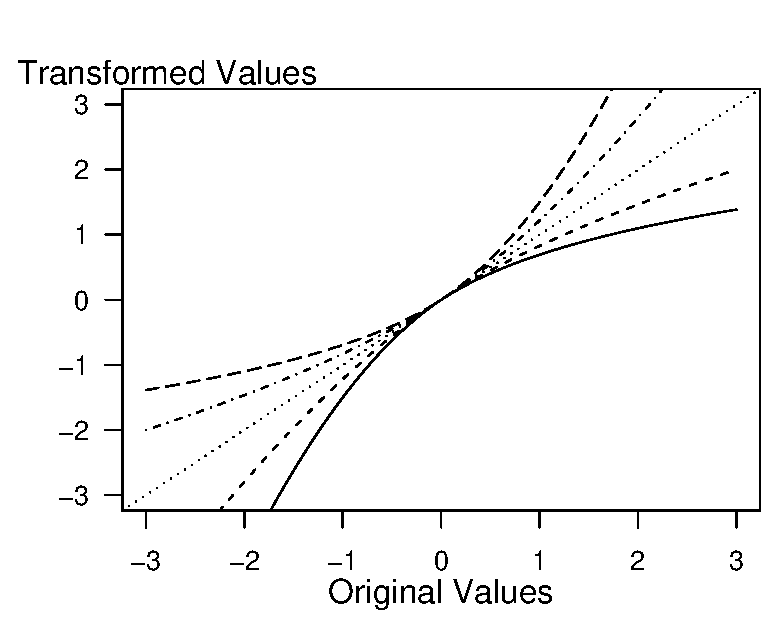
\includegraphics[width=.6\textwidth]
        {Chapter17FatTail/F17Transform.eps}
\caption{\label{F17:Transform} \small Yeo-Johnson Transformations.
From bottom to top, the curves correspond to $\lambda =0,0.5,1,1.5$
and 2.}
\end{figure}

Both the John and Draper as well as the Yeo and Johnson families are
based on power transforms. An alternative family, due to Burbidge
and Magee (1988), is a modification of the inverse hyperbolic sine
transformation. This family is given by:
\begin{equation*}
y^{(\lambda)}=\sinh^{-1}(\lambda y)/\lambda .
\end{equation*}\index{transformations!Burbidge-Magee family}


\section{Generalized Linear Models}\label{S17:GLMs}\index{regression model!generalized linear model, $GLM$}

As introduced in Chapter 13, the generalized linear model (GLM)
method has become popular in financial and actuarial statistics. An
advantage of this methodology is the ability to fit distributions
with tails heavier than the normal distribution. In particular, GLM
methods are based on the exponential family that includes the
normal, gamma and inverse gaussian distributions. As we will see in
Section \ref{S17:FatSubsection}, it is customary to think of the
gamma distribution as having intermediate tails and the inverse
gaussian as having heavy tails compared to the thin-tailed normal
distribution.

The idea of a GLM is to map a linear systematic component
$\mathbf{x}^{\prime }\boldsymbol \beta$\ into the mean of the
variable of interest through a known function. Thus, GLMs provide a
natural way to include covariates into the modeling. With a GLM, the
variance is not required to be constant as in the linear model, but
is a function of the mean. Once the distribution family and link
function have been specified, estimation of GLM regression
coefficients depends only on the mean and thus is robust to some
model distribution mis-specifications. This is both a strength and
weakness of the GLM approach. Although more flexible than the linear
model, this approach does not handle many of the long-tail
distributions traditionally used for modeling insurance data. Thus,
in Section \ref{S17:GenrlDistns} we will present more flexible
distributions.


\subsection{What is ``Fat-Tailed?''}\label{S17:FatSubsection}

Many analysts begin discussions of tail heaviness through skewness
and kurtosis coefficients. \emph{Skewness} measures the lack of
symmetry, or lop-sidedness, of a distribution. It is typically
quantified by the third standardized moment, \newline
$\mathrm{E}(y-\mathrm{E~}y)^3/ (\mathrm{Var~}y)^{3/2}.$
\emph{Kurtosis} measures tail heaviness, or its converse,
``peakedness.'' It is typically quantified by the fourth
standardized moment minus 3, \newline $\mathrm{E}(y-\mathrm{E~}y)^4/
(\mathrm{Var~}y)^{2} -3.$  The ``minus 3'' is to center discussions
around the normal distribution; that is, for a normal distribution,
one can check that  \newline
$\mathrm{E}(y-\mathrm{E~}y)^4/(\mathrm{Var~}y)^{2} =3.$
Distributions with positive kurtosis are called \emph{leptokurtic}
whereas those with negative kurtosis are called \emph{platykurtic}.
These definitions focus heavily on the normal that has traditionally
been viewed as the benchmark distribution.

For many actuarial and financial applications, the normal
distribution is not an appropriate starting point and so we seek
other definitions of ``fat-tail.'' In addition to moments, the size
of the tail can be measured using a density (or mass, for discrete
distributions) function, the survival function, or a conditional
moment. Typically, the measure would be used to compare one
distribution to another.

For example, comparing the right tails of the normal to a gamma
density function, we
have\index{distributions!gamma}\index{distributions!normal}
\begin{eqnarray*}
\frac{\mathrm{f}_{normal}\left( y\right) }{\mathrm{f}_{gamma}\left( y\right)
} &=&\frac{\sqrt{2\pi \sigma ^{2}}\exp \left( -\left( y-\mu \right)
^{2}/(2\sigma ^{2})\right) }{\left[ \lambda ^{\alpha }\Gamma \left( \alpha
\right) \right] ^{-1}y^{\alpha -1}\exp \left( -y/\lambda \right) } \\
&=&C_1\mathit{\exp }\left( -(\alpha -1)\ln y+y/\lambda -\left( y-\mu
\right) /(2\sigma ^{2})\right) \rightarrow 0,
\end{eqnarray*}
as $y\rightarrow \infty $, indicating that the gamma has a heavier, or
fatter, tail than the normal.

Both the normal and the gamma are members of the exponential family
of distributions. For comparison with another member of this family,
the inverse gaussian distribution,
consider\index{distributions!inverse gaussian}
\begin{eqnarray*}
\frac{\mathrm{f}_{gamma}\left( y\right)
}{\mathrm{f}_{invGaussian}\left( y\right) } &=&\frac{\left[ \lambda
^{\alpha }\Gamma \left( \alpha \right) \right] ^{-1}y^{\alpha
-1}\exp \left( -y/\lambda \right) }{\sqrt{\theta /(2\pi y^{3})}\exp
\left( -\theta \left( y-\mu \right) ^{2}/(2y\mu
^{2})\right) } \\
&=&C_2\mathit{\exp }\left( (\alpha +1/2)\ln y-y/\lambda +\theta
\left( y-\mu \right) ^{2}/(2y\mu ^{2}))\right) .
\end{eqnarray*}
As $y\rightarrow \infty $, this ratio tends to zero for $\theta
/(2\mu ^{2})<\lambda ,$\ indicating that the inverse gaussian can
have a heavier tail than the gamma.

For a distribution that is not a member of the exponential family,
consider the Pareto distribution. Similar calculations
show\index{distributions!Pareto}
\begin{eqnarray*}
\frac{\mathrm{f}_{gamma}\left( y\right) }{\mathrm{f}_{Pareto}\left( y\right)
} &=&\frac{\left[ \lambda ^{\alpha }\Gamma \left( \alpha \right) \right]
^{-1}y^{\alpha -1}\exp \left( -y/\lambda \right) }{\alpha \theta ^{-\alpha
}\left( y+\theta \right) ^{-\alpha -1}} \\
&=&C_3\mathit{\exp }\left( (\alpha -1)\ln y-y/\lambda +\left( \alpha
+1\right) \ln \left( y+\theta \right) \right) \rightarrow 0,
\end{eqnarray*}
as $y\rightarrow \infty $, indicating that the Pareto has a heavier tail
than the gamma.

The ratio of densities is an easily interpretable measure for
comparing the tail heaviness of two distributions. Because densities
and survival functions have a limiting value of zero, by
L'H\^{o}pital's rule the ratio of survival functions is equivalent
to the ratio of densities. That is,
\begin{equation*}
\lim_{y\rightarrow \infty }\frac{\mathrm{S}_1\left( y\right)
}{\mathrm{S} _2\left( y\right) }=\lim_{y\rightarrow \infty
}\frac{\mathrm{S} _1^{\prime }\left( y\right) }{\mathrm{S}_2^{\prime
}\left( y\right) } = \lim_{y\rightarrow \infty }\frac{\mathrm{f}_1
\left( y\right) }{\mathrm{f}_2 \left( y\right) }.
\end{equation*}
This provides another motivation for using this measure.


\subsection{Application: Wisconsin Nursing Homes}\label{Ex:NursHome}

\empexjed{WiscNursingHome}\index{datasets!nursing home utilization}

Nursing home financing has drawn the attention of policymakers and
researchers for the past several decades. With aging populations and
increasing life expectancies, expenditures on nursing homes and
demands of long term care are expected to increase in the future. In
this section, we analyze the data of 349 nursing facilities in the
State of Wisconsin in the cost report year 2001.

The state of Wisconsin Medicaid program funds nursing home care for
individuals qualifying on the basis of need and financial status.
Most, but not all, nursing homes in Wisconsin are certified to
provide Medicaid-funded care. Those that do not accept Medicaid are
generally paid directly by the resident or the resident's insurer.

Similarly, most, but not all, nursing facilities are certified to
provide Medicare-funded care. Medicare provides post-acute care for
100 days following a related hospitalization. Medicare does not fund
care provided by intermediate care facilities to individuals with
developmental disabilities. As part of the conditions for
participation, Medicare-certified nursing homes must file an annual
cost report to the Wisconsin Department of Health and Family
Services summarizing the volume and cost of care provided to all of
its residents, Medicare-funded and otherwise.

Nursing homes are owned and operated by a variety of entities,
including the state, counties, municipalities, for-profit businesses
and tax-exempt organizations. Private firms often own several
nursing homes.  Periodically, facilities may change ownership and,
less frequently, ownership type.

Typically, utilization of nursing home care is measured in patient
days. Facilities bill the fiscal intermediary at the end of each
month for total patient days incurred in the month, itemized by
resident and level of care. Projections of patient days by facility
and level of care play a key role in the annual process of updating
facility rate schedules. Rosenberg et al. (2007) provides additional
discussion.

\subsubsection*{Summarizing the Data}

After examining the data, we found some minor variations in the
number of days that a facility was open, primarily due to openings
and closing of facilities. Thus, to make utilization more comparable
among facilities, we examine TPY, defined to be the total number of
patient days divided by the number of days the facility was open;
this has a median value of 81.99 per facility.

Table \ref{T17:SummStatsWiscNursHome} describes the variables that
will be used to explain the distribution of TPY. More than half of
the facilities have self funding of insurance. Approximately
$90.5\%$ of the facilities are Medicare Certified. Regarding the
organizational structure, about half $(51.9\%)$ are run on a
for-profit basis, and about one third $(37.5\%)$ are organized as
tax exempt and the remainder are governmental organizations. The tax
exempt facilities have the highest median occupancy rates. Slightly
more than half of the facilities are located in an urban environment
(53.3\%).

\begin{table}[h]
\scalefont{0.9} \caption{\label{T17:SummStatsWiscNursHome} Nursing
Home Descriptive Statistics}
\begin{tabular}{llrr}\hline
Variable & Description \\
\hline TPY & Total person years (median 81.89) &  & \\\hline
\multicolumn{4}{l}{Continuous Explanatory Variables}\\
NumBed & Number of beds (median 90) &  & \\
SqrFoot & Nursing home net square footage. &  & \\
 & \ \ \ \ \ \ (in
thousands, median 40.25) &  & \\
\hline
\multicolumn{2}{l}{Categorical Explanatory Variables}& Percentage & Median TPY\\
POPID & \multicolumn{3}{l}{Nursing home identification number} \\
SelfIns & Self Funding of Insurance &  & \\
 & Yes & 62.8 & 88.40\\
 &  No & 37.2 & 67.84\\
MCert & Medicare Certified & & \\
& Yes & 90.5 & 84.06\\
 & No & ~9.5 & 53.38\\
Organizational & Pro (for profit)         & 51.9 & 77.23\\
  ~~~Structure              & TaxExempt (tax exempt)   & 37.5 & 81.13\\
                         & Govt (governmental unit) & 10.6 & 106.70\\
Location & Urban & 53.3 & 91.55\\
         & Rural & 46.7 & 74.12\\
\hline
\end{tabular}
\scalefont{1.1111}
\end{table}



\subsubsection*{Fitting Generalized Linear Models}

Figure \ref{F17:NursHist} shows the distribution of the dependent
variable TPY. From this figure, we see clear evidence of the
right-skewness of the distribution. One option would be to take a
transform as described in Section \ref{S17:Transforms}. Rosenberg et
al. (2007) explored this option using a logarithmic transformation.


\begin{figure}[htp]
  \begin{center}
    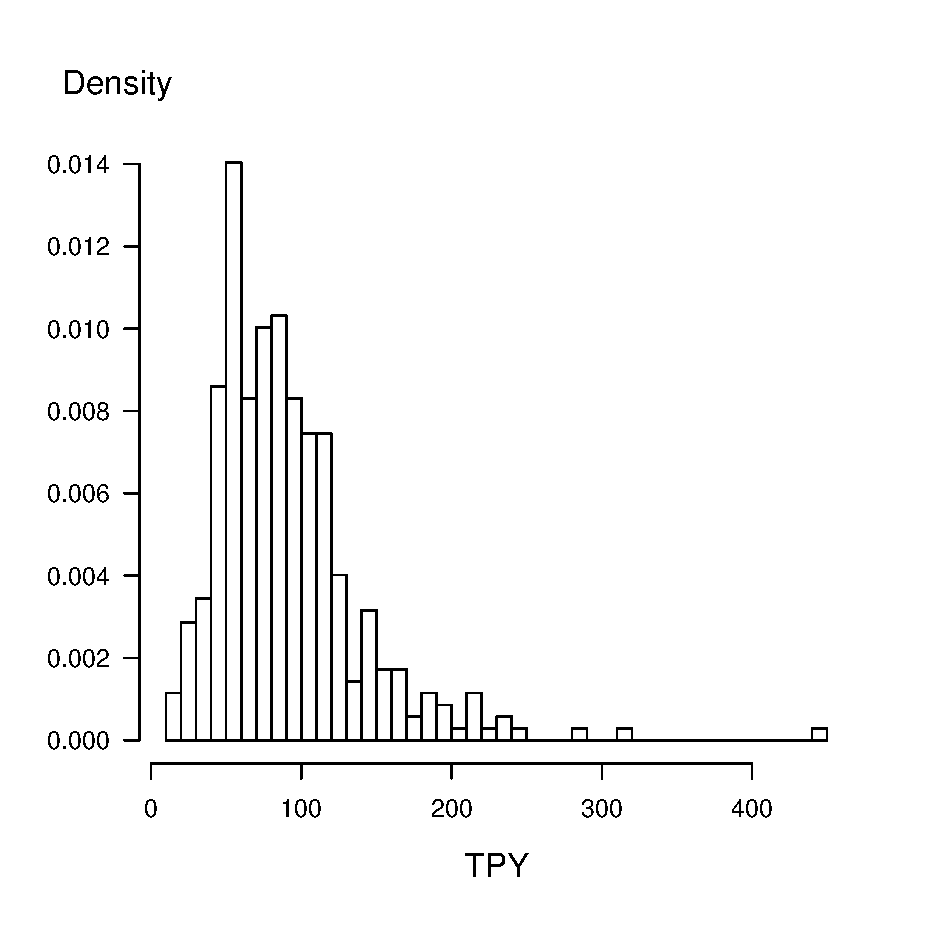
\includegraphics[width=.6\textwidth]{Chapter17FatTail/F17NursHist.eps}
    \caption{\label{F17:NursHist} \small Histogram of TPY.
    This plot demonstrates the right skewness of the distribution.}
  \end{center}
\end{figure}

Another option is to directly fit a skewed distribution to the data.
Figure \ref{F17:Disqq} presents the $qq$ plots of the gamma and
inverse gaussian distributions. The data fall fairly close to the
line in both panels, meaning both models are reasonable choices. The
normal $qq$ plot, not shown here, indicates that the normal
regression model is not a reasonable fit.


\begin{figure}[htp]
  \begin{center}
    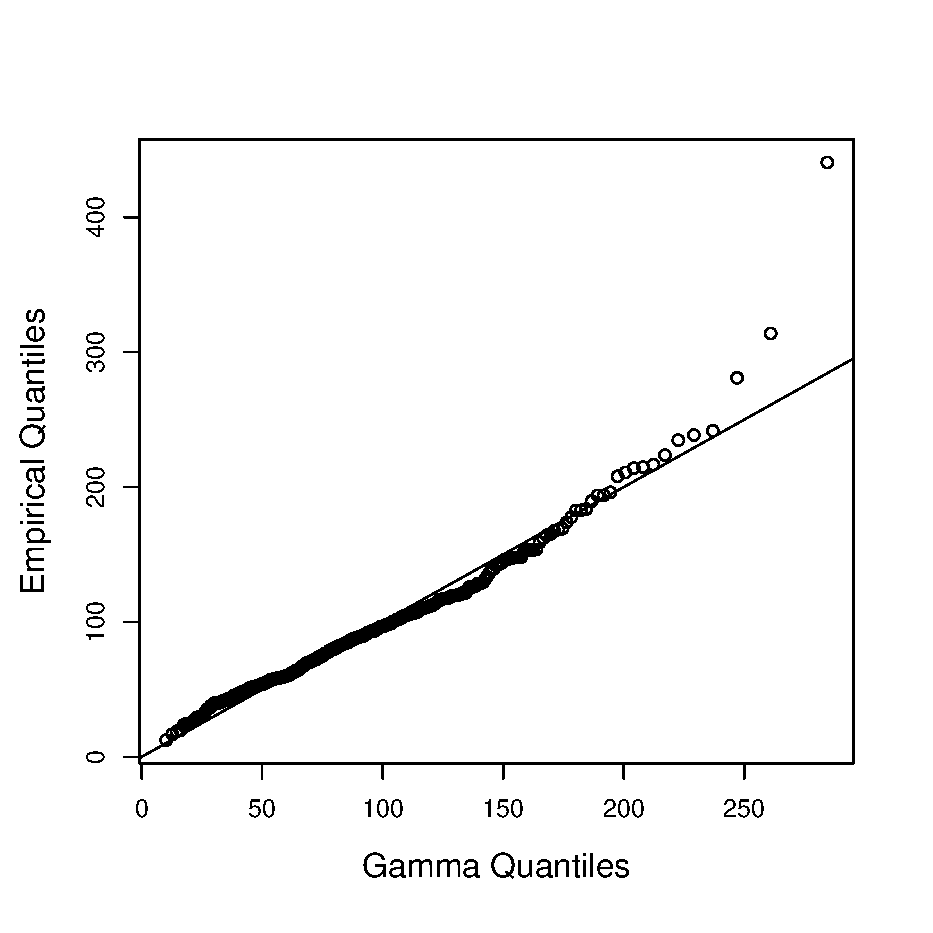
\includegraphics[width=0.45\textwidth]  {Chapter17FatTail/F17GammaQQ.eps} \hfill
    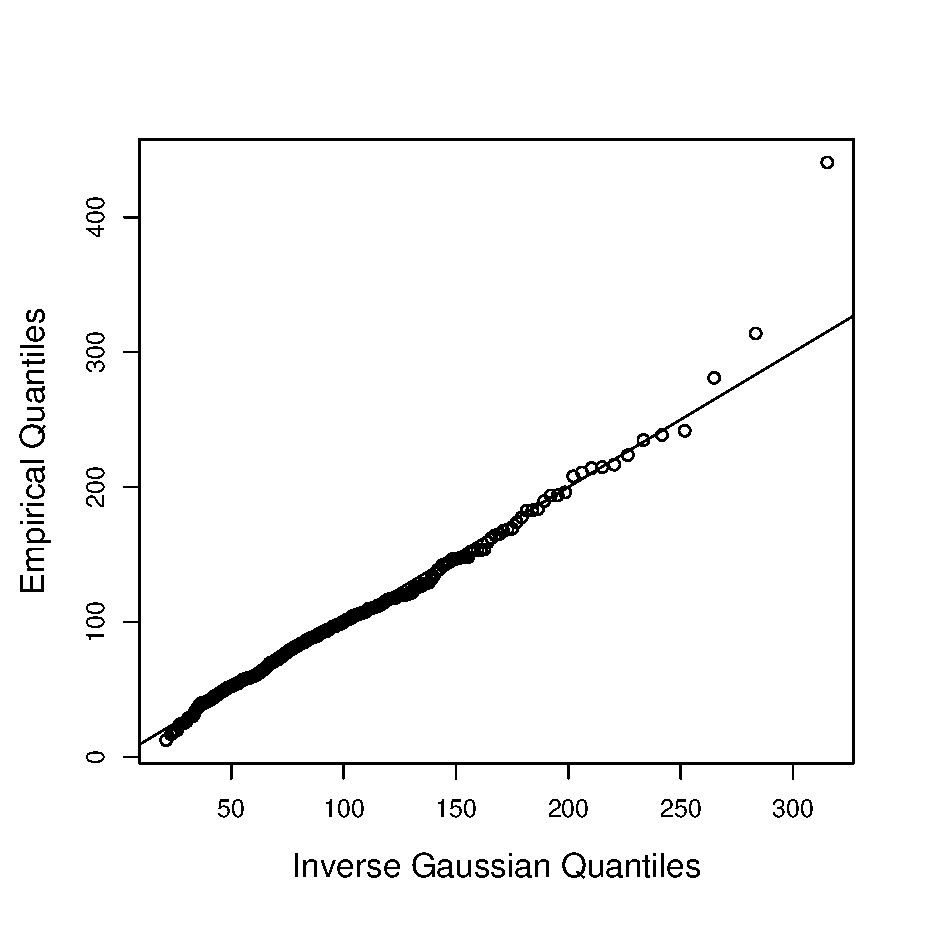
\includegraphics[width=0.45\textwidth]{Chapter17FatTail/F17InvGausQQ.eps}
    \caption{\label{F17:Disqq} \small $qq$ Plots of TPY for the Gamma and Inverse Gaussian Distributions.}
    \end{center}
\end{figure}


We fit the generalized linear models using the gamma and inverse
gaussian distributions. In both models, we choose the logarithmic
link function. The linear systematic component that is common to
each model is
\begin{eqnarray} \label{E17:reg1}
&& \eta = \beta_0 + \beta_1 \ln(\text{NumBed}) + \beta_2
\ln(\text{SqrFoot}) +
\beta_3 \text{Pro}  \\
&& + \beta_4 \text{TaxExempt} + \beta_5 \text{SelfIns} + \beta_6
\text{MCert} + \beta_7 \text{Urban}. \notag
\end{eqnarray}


Table \ref{T17:GLMWiscNursHome} summarizes the parameter estimates
of the models. By comparing the BIC statistics, or the AIC and
log-likelihood in that the number of estimated parameters and the
sample size in both models are identical, we find the gamma model
performs better than the inverse gaussian. As anticipated, the
coefficient for the size variable NumBed is positive and
significant. The only other variable that is statistically
significant is the SqrFoot variable, and this only in the gamma
model.



\begin{table}[h]\scalefont{0.9}
\caption{\label{T17:GLMWiscNursHome} Fitted Nursing Home Generalized
Linear Models}
\begin{tabular}{l|rrrr}
\hline
& \multicolumn{2}{|c}{Gamma} & \multicolumn{2}{c}{Inverse Gaussian} \\
Variables & Estimate & $t$-ratio & Estimate & $t$-ratio\\
\hline
Intercept    & -0.159 & -3.75 & -0.196 & -4.42 \\
ln(NumBed)   & 0.996  & 66.46 & 1.023 & 65.08 \\
ln(SqrFoot)  & 0.026  & 2.07  & 0.003 & 0.19 \\
SelfIns      & 0.006  & 0.75  & 0.003 & 0.27 \\
MCert        & -0.008 & -0.55  & -0.008 & -0.57 \\
Pro          & 0.004  & 0.29  & 0.007 & 0.36 \\
TaxExempt    & 0.018  & 1.28  & 0.021 & 1.12 \\
Urban        & -0.011 & -1.25 & -0.006 & -0.64 \\
Scale        &    165.64&   & 0.0112  \\ \hline
\multicolumn{2}{l}{Goodness of Fit Statistics}  \\
Log Likelihood & \multicolumn{2}{r}{-1,131.24} & \multicolumn{2}{r}{-1,218.15}  \\
AIC &\multicolumn{2}{r}{2,280.47} & \multicolumn{2}{r}{2,454.31}\\
 BIC & \multicolumn{2}{r}{2,315.17}  & \multicolumn{2}{r}{2,489.00}  \\ \hline
\end{tabular}\scalefont{1.1111}
\end{table}


Figure \ref{F17:res} presents the plots of deviance residuals
against the fitted value of TPY for the gamma and inverse gaussian
models. No patterns are found in the plots, supporting the position
that these models are reasonable fits to the data.

\begin{figure}[htp]
  \begin{center}
    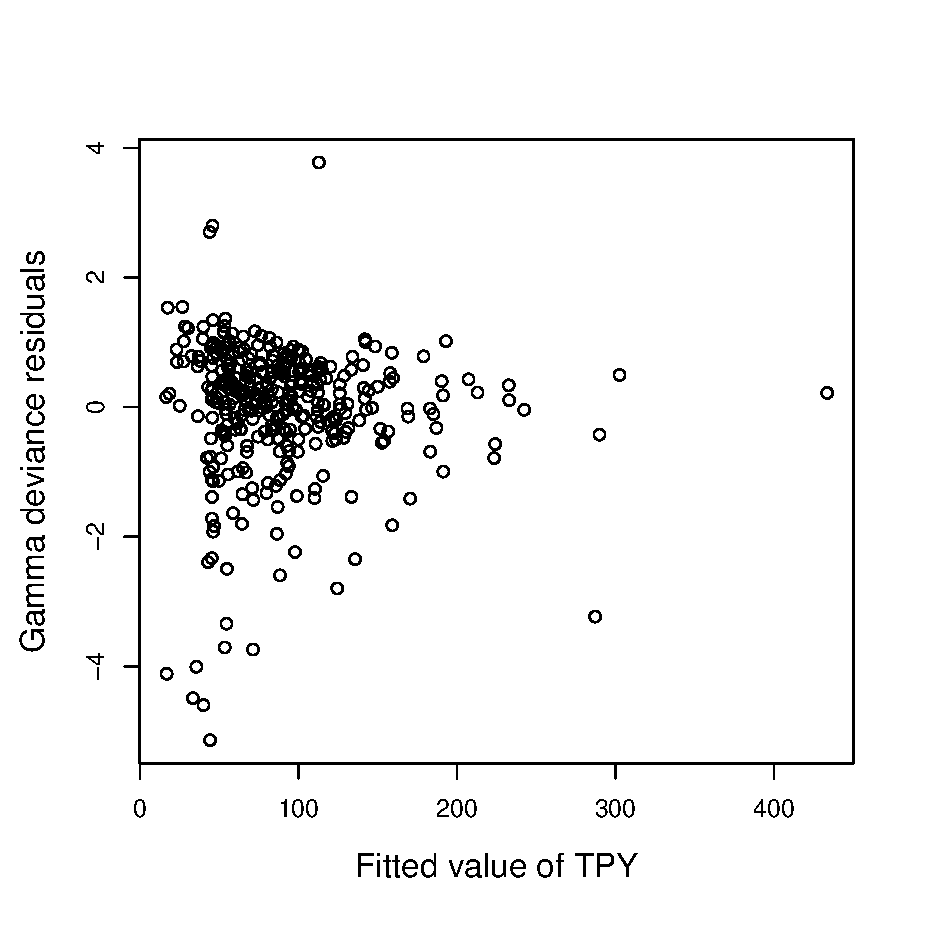
\includegraphics[width=0.45\textwidth]  {Chapter17FatTail/F17GamResids.eps} \hfill
    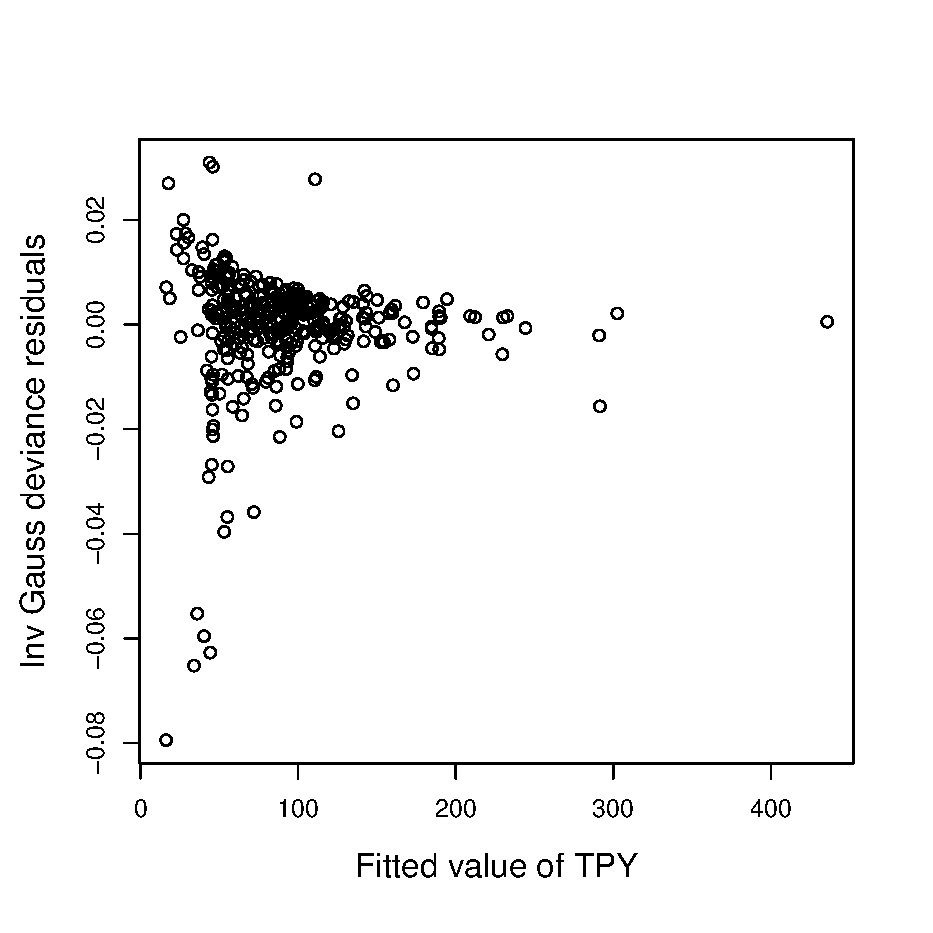
\includegraphics[width=0.45\textwidth]{Chapter17FatTail/F17InvGaussResids.eps}
 \caption{\label{F17:res} \small Plots of Deviance Residuals versus Fitted Values
             for the Gamma and Inverse Gaussian Models.}
     \end{center}
\end{figure}


\section{Generalized Distributions}\label{S17:GenrlDistns}


Another approach for handling fat-tailed regression data is to use
parametric distributions, such as those from the survival modeling.
Although survival analysis focuses on censored data, the methods can
certainly be applied to complete data. In Section 14.3 we introduced
an accelerated failure time (AFT) model. The AFT is a log
location-scale model, so that $\ln (y)$ follows a parametric
location-scale density distribution in the form
$\mathrm{f}(y)=\mathrm{f}_0\left( (y-\mu )/\sigma \right) /\sigma $,
where $\mu $ and $\sigma >0$ are location and scale parameters, and
$\mathrm{f}_0$ is the standard form of the distribution. The
Weibull, lognormal and loglogistic distributions are commonly used
lifetime distributions that are special cases of the AFT framework.

For fitting fat-tailed distributions of interest in actuarial
science, we consider the following minor variation, and examine
distributions from the relation
\begin{equation}\label{E17:GenDistEq}
\ln y = \mu + \sigma \ln y_0.
\end{equation}
As before, the distribution associated with $y_0$ is a standard one
and we are interested in the distribution of the random variable
$y$. Two important special cases are the generalized gamma and the
generalized beta of the second kind. These distributions have been
used extensively in modeling insurance data, see for example,
Klugman et al. (2008), although most applications have not utilized
regression covariates.

\index{distributions!generalized
gamma}\index{distributions!generalized beta of the second kind
distribution, $GB2$}

The \emph{generalized gamma distribution }is obtained when $y_0$\
has a gamma distribution with shape parameter $\alpha$ and scale
parameter 1. When including limiting distributions (such as allowing
coefficients to become arbitrarily large), it includes the
exponential, Weibull, gamma, and lognormal distributions as special
cases. Therefore, it can be used to discriminate between the
alternate models. The generalized gamma distribution is also known
as the transformed gamma distribution (Klugman et al., 2008).

When $y_0$ has a distribution that is the ratio of two gammas, then
$y$ is said to have a \emph{generalized beta of the second kind
distribution,} commonly known by the acronym \emph{GB2}.
Specifically, we assume that $y_0 = Gamma_1/Gamma_2$, where
$Gamma_i$ has a gamma distribution with shape parameter $\alpha_i$
and scale parameter 1, $i=1,2$, and that $Gamma_1$ and $Gamma_2$ are
independent. Thus, the GB2 family has four parameters ($\alpha_1$,
$\alpha_2$, $\mu$ and $\sigma$) compared to the three parameter
generalized gamma distribution. When including limiting
distributions, the GB2 encompasses the generalized gamma (by
allowing $\alpha_2 \rightarrow \infty)$ and hence the exponential,
Weibull, and so forth. It also encompasses the Burr Type 12 (by
allowing $\alpha_1 = 1$), as well as other families of interest,
including the Pareto distributions.

The distribution of $y$ from equation (\ref{E17:GenDistEq}) contains
location parameter $\mu$, scale parameter $\sigma$ and additional
parameters that describe the distribution of $y_0$. In principle,
one could allow for any distribution parameter to be a function of
the covariates. However, following this principle would lead to a
large number of parameters; this typically yields computational
difficulties as well as problems of interpretations. To limit the
number of parameters, it is customary to assume that the parameters
from $y_0$ do not depend on covariates. It is natural to allow the
location parameter to be a linear function of covariates so that
$\mu =\mu \left( \mathbf{x}\right)= \mathbf{x}^{\prime } \boldsymbol
\beta$. One may also allow the scale parameter $\sigma$ to depend on
$\mathbf{x}$. For $\sigma $ positive, a common specification is $
\sigma =\sigma (\mathbf{x})$ = exp$(\mathbf{x}^{\prime }\boldsymbol
\beta_{\sigma })$, where $\boldsymbol \beta_{\sigma }$\ are
regression coefficients associated with the scale parameter. Other
parameters are typically held fixed.

The interpretability of parameters is one reason to hold the scale
and other non-location parameters fixed. By doing this, it is
straightforward to show that the regression function is of the form
\begin{equation*}
\mathrm{E}\left( y|\mathbf{x}\right) =C\exp \left( \mu \left(
\mathbf{x} \right) \right) =C~e^{\mathbf{x}^{\prime }\boldsymbol
\beta},
\end{equation*}
where the constant $C$ is a function of other (non-location) model
parameters. Thus, one can interpret the regression coefficients in
terms of a proportional change (an \emph{elasticity} in economics).
That is, $\partial \left[ \ln \mathrm{E}(y) \right] /\partial x_k=
\beta_k.$\index{actuarial \& financial terms and
concepts!elasticity}

Another reason for holding non-location parameters fixed is the ease
of computing sensible residuals and using these residuals to assist
with model selection. Specifically, with equation
(\ref{E17:GenDistEq}), one can compute residuals of the form
\begin{equation*}
r_i = \frac{\ln y_i-\widehat{\mu}_i }{\widehat{\sigma }},
\end{equation*}
where $\widehat{\mu}_i$\ and $\widehat{\sigma }$\ are maximum
likelihood estimates. For large data sets, we may assume little
estimation error so that $ r_i \approx (\ln y_i - \mu_i) /\sigma,$
and the quantity on the right-hand side has a known distribution.

To illustrate, consider the case when $y$ follows a GB2
distribution. In this case,
\begin{equation*}
y_0 = \frac{Gamma_1}{Gamma_2}= \frac{\alpha_1}{\alpha_2} \times
\frac{Gamma_1/(2\alpha_1)}{Gamma_2/(2\alpha_2)} =
\frac{\alpha_1}{\alpha_2} \times F ,
\end{equation*}
where $F$ has an $F$-distribution with numerator and denominator
degrees of freedom $df_1 = 2 \alpha_1$ and $df_2 = 2 \alpha_2$.
Then, $\exp(r_i) \approx (\alpha_1 /\alpha_2) F_i $, so that the
exponentiated residuals should have an approximate
\textit{F}-distribution (up to a scale parameter). This fact allows
us to compute quantile-quantile (\emph{qq}) plots to assess model
adequacy graphically.

To illustrate, we consider a few insurance related examples that use
fat-tailed regression models. McDonald and Butler (1990) discussed
regression models including those commonly used as well as the GB2
and generalized gamma distribution. They applied the model to the
duration of poverty spells and found that the GB2 improved model
fitting significantly over the lognormal. Beirlant et al. (1998)
proposed two Burr regression models, and applied them to portfolio
segmentation for fire insurance. The Burr is a an extension of the
Pareto distribution, although still a special case of the GB2.
Manning, Basu and Mullahy (2005) applied the generalized gamma
distribution to inpatient expenditures using the data from a study
of hospitals conducted at the University of Chicago.

Because the regression model is fully parametric, maximum likelihood
is generally the estimation method of choice. If $y$ follows a GB2
distribution, straight-forward calculations show that its density
can be expressed as
\begin{equation} \label{E17:GB2}
f(y; \mu, \sigma, \alpha_1, \alpha_2) = \frac{[\exp(
z)]^{\alpha_{1}}}{y |\sigma| B(\alpha_1, \alpha_2) [1 + \exp(z)
]^{\alpha_1 + \alpha_2} },
\end{equation}
where $z= (\ln y - \mu)/{\sigma}$ and B($\cdot,\cdot$) is the beta
function, defined as $\text{B}(\alpha_1, \alpha_2) =
\Gamma(\alpha_1)\Gamma(\alpha_2)/\Gamma(\alpha_1+\alpha_2)$. This
density can be used directly in likelihood routines of many
statistical packages. As described in Section 11.9, the method of
maximum likelihood automatically provides:
\begin{itemize}
\item standard errors for the parameter estimates,

\item methods of model selection via likelihood ratio testing and

\item goodness of fit statistics such as AIC and BIC.
\end{itemize}



\subsection*{Application:Wisconsin Nursing Homes}\index{datasets!nursing home utilization}

In the fitted generalized linear models summarized in Table
\ref{T17:GLMWiscNursHome}, we saw that the coefficients associated
with ln(NumBed) were close to one. This suggest identifying
ln(NumBed) as an \emph{offset variable}, that is, forcing the
coefficient associated with ln(NumBed) to be 1. For another modeling
strategy, it also suggests rescaling the dependent variable by
NumBed. This is sensible because we used a logarithmic link function
so that the expected value of TPY is proportional to NumBed.
Pursuing this approach, we now define the annual occupancy rate
(Rate) to be
\begin{equation}
\text{Occupancy Rate} = \frac{\text{Total Patient
Days}}{\text{Number of Beds} \times \text{Days Open}} \times 100.
\end{equation}
This new dependent variable is easy to interpret - it measures the
percentage of beds being used on any given day. Occupancy rates were
calculated using the average number of licensed beds within a cost
report year rather than the number of licensed beds on a specific
day. This gives rise to a few occupancy rates greater than 100.

One difficulty of using occupancy rates is that its distribution
cannot reasonably be approximated by a member of the exponential
family. Figure \ref{F17:GB2Nurse} shows a smoothed histogram of the
Rate variable (using a kernel smoother); this distribution is
\emph{left}-skewed. Superimposed on it with the dotted line is the
inverse gaussian distribution where the parameters were fit without
covariates, using method of moments. The gamma and normal
distributions are very close to the inverse gaussian, and hence are
not shown here. In contrast, the fitted (also without covariates)
GB2 distribution shown in Figure \ref{F17:GB2Nurse} captures
important parts of the distribution; in particular, it captures the
peakedness and left-skewness.



\begin{figure}[htp]
  \centering
    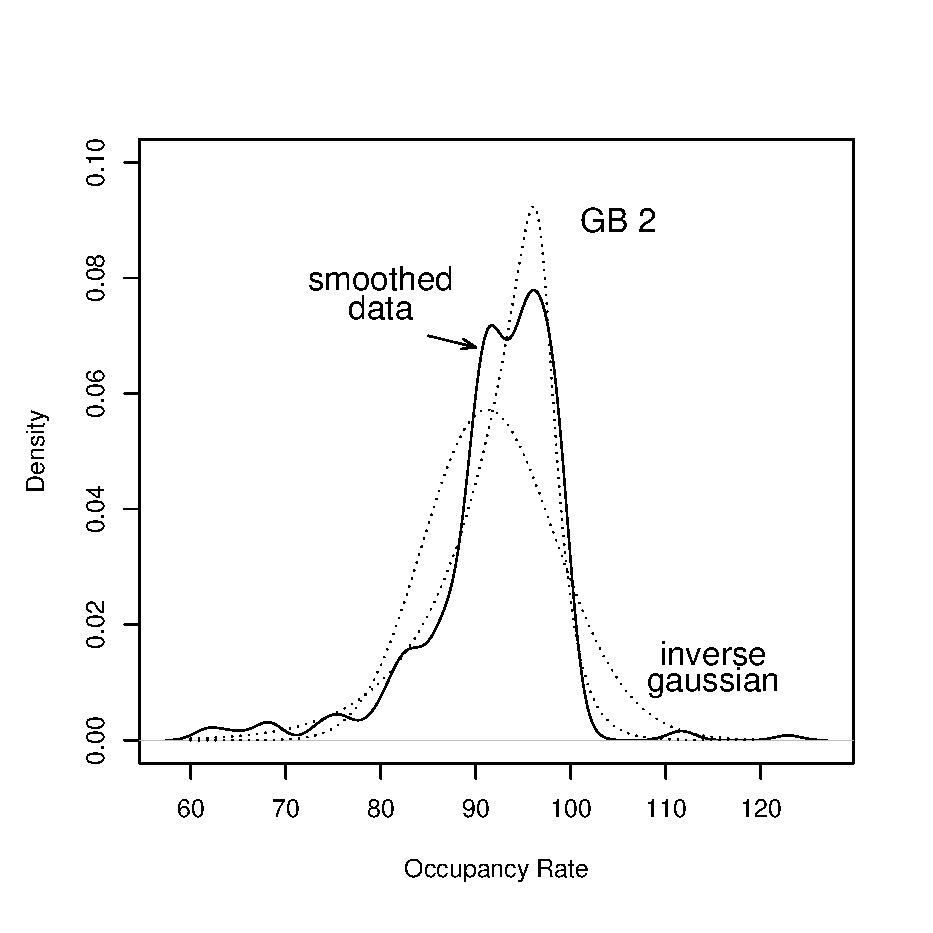
\includegraphics[width=.6\textwidth]
        {Chapter17FatTail/F17GB2Nurse.eps}
\caption{\label{F17:GB2Nurse} \small Nursing Home Densities. The
empirical version, based on a kernel density estimate, is compared
to fitted GB2 and inverse gaussian densities.}
\end{figure}\index{density estimation!kernel}


The GB2 distribution was fit using maximum likelihood with the same
covariates as in Table \ref{T17:GLMWiscNursHome}. Specifically, we
used location parameter $\mu = \exp(\eta)$, where $\eta$ is
specified in equation (\ref{E17:reg1}). As is customary in
likelihood estimation, we reparameterized the scale and two shape
parameters, $\sigma$, $\alpha_1$ and $\alpha_2$, to be transformed
on the log scale so that they could range over the whole real line.
In this way, we avoided boundary problems that could arise when
trying to fit models with negative parameter values. Table
\ref{T17:GModelsWiscNursHome} summarizes the fitted model.
Unfortunately, for this fitted model, none of the explanatory
variables turned out to be statistically significant. (Recall that
we rescaled by number of beds, a very important explanatory
variable.)



\begin{table}[h]\scalefont{0.9}
\caption{\label{T17:GModelsWiscNursHome} Wisconsin Nursing Home
Generalized Models Fits}
\begin{tabular}{lrrrr}
\hline & \multicolumn{2}{c}{Generalized Gamma}
&\multicolumn{2}{c}{GB2} \\
\hline Variables & Estimate & \textit{t}-ratio &Estimate &
\textit{t}-ratio \\ \hline
Intercept   &      4.522 &      78.15 &      4.584 &     198.47 \\
ln(NumBed)  &     -0.027 &      -2.06 &     -0.010 &      -1.17 \\
ln(SqrFoot) &      0.031 &       2.89 &      0.010 &       1.28 \\
SelfIns     &      0.003 &       0.44 &     -0.001 &      -0.25 \\
MCert       &     -0.010 &      -0.81 &     -0.010 &      -1.30 \\
Pro         &     -0.021 &      -1.46 &     -0.002 &      -0.20 \\
TaxExempt   &     -0.007 &      -0.48 &      0.015 &       1.66 \\
Urban       &     -0.014 &      -1.78 &     -0.003 &      -0.60 \\
\hline      & Estimate   & Std Error  & Estimate   & Std Error \\
$\ln \sigma$    &     -2.406 &     0.131 &     -5.553 &      1.716 \\
$\ln \alpha_1$  &      0.655 &     0.236 &     -2.906 &      1.752 \\
$\ln \alpha_2$  &            &            &     -1.696 &     1.750 \\
\hline
Log-Likelihood & \multicolumn{2}{c}{-1,148.135} &  \multicolumn{2}{c}{-1,098.723} \\
AIC            & \multicolumn{2}{c}{~2,316.270} &  \multicolumn{2}{c}{~2,219.446} \\
BIC            & \multicolumn{2}{c}{~2,319.296} &  \multicolumn{2}{c}{~2,223.822}\\
\hline
\end{tabular}
\scalefont{1.1111}
\end{table}


To further assess the model fit, Figure \ref{F17:GB2ResidAnalysis}
shows residuals from this fitted model. For these figures, residuals
are computed using $r_i = (\ln y_i-\widehat{\mu}_i)/\widehat{\sigma
}.$ The left-hand panel shows the residuals versus fitted values
($\exp(\widehat{\mu}_i)$), no apparent patterns are evident in this
display. The right-hand panel is a $qq$ plot of residuals, where the
reference distributions is the logarithmic $F$-distribution (plus a
constant) described above. This figure shows some discrepancies for
smaller values of nursing homes. Because of this, Table
\ref{T17:GModelsWiscNursHome} also reports fits from the generalized
gamma model. This fit is more pleasing in the sense that two of the
explanatory variable are statistically significant. However, from
the goodness of fit statistics, we see that the GB2 is a better
fitting model. Note that the goodness of fit statistics for the
generalized gamma model are not directly comparable with the gamma
regression fits in Table \ref{T17:GLMWiscNursHome}; this is only
because the dependent variable differs by the scale variable
NumBeds.


\begin{figure}[htp]
  \begin{center}
    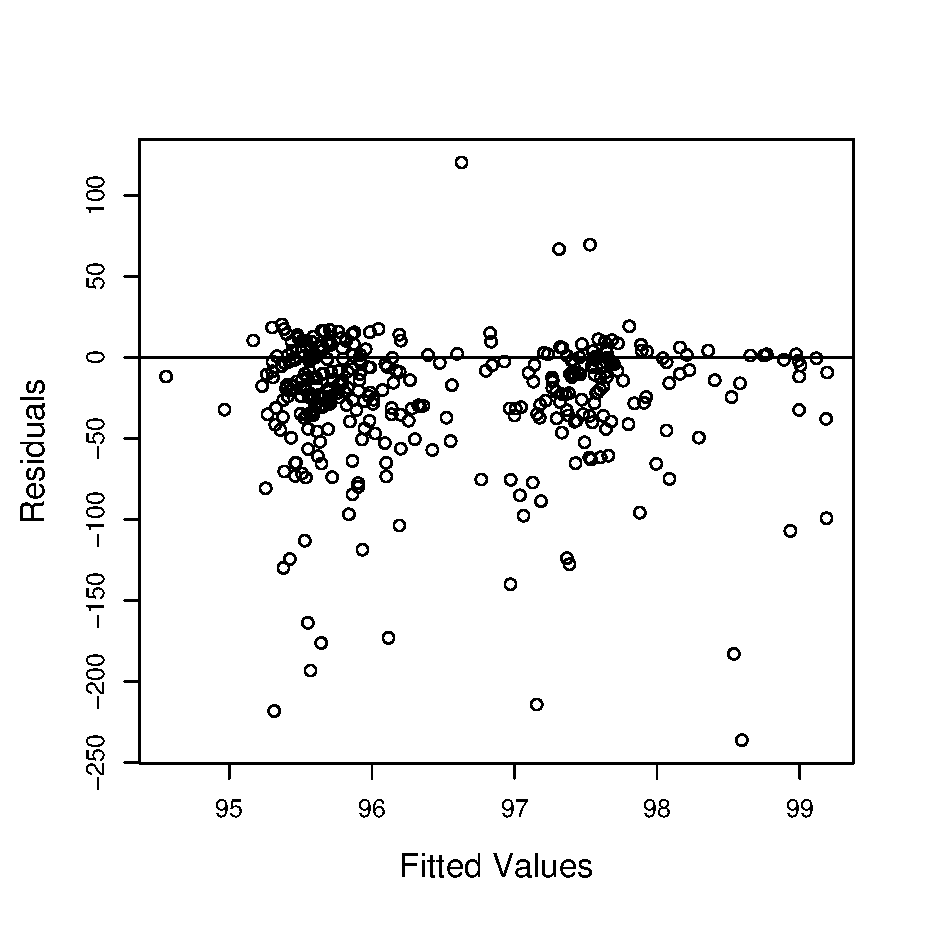
\includegraphics[width=0.45\textwidth]  {Chapter17FatTail/F17GB2FITRESIDS.eps} \hfill
    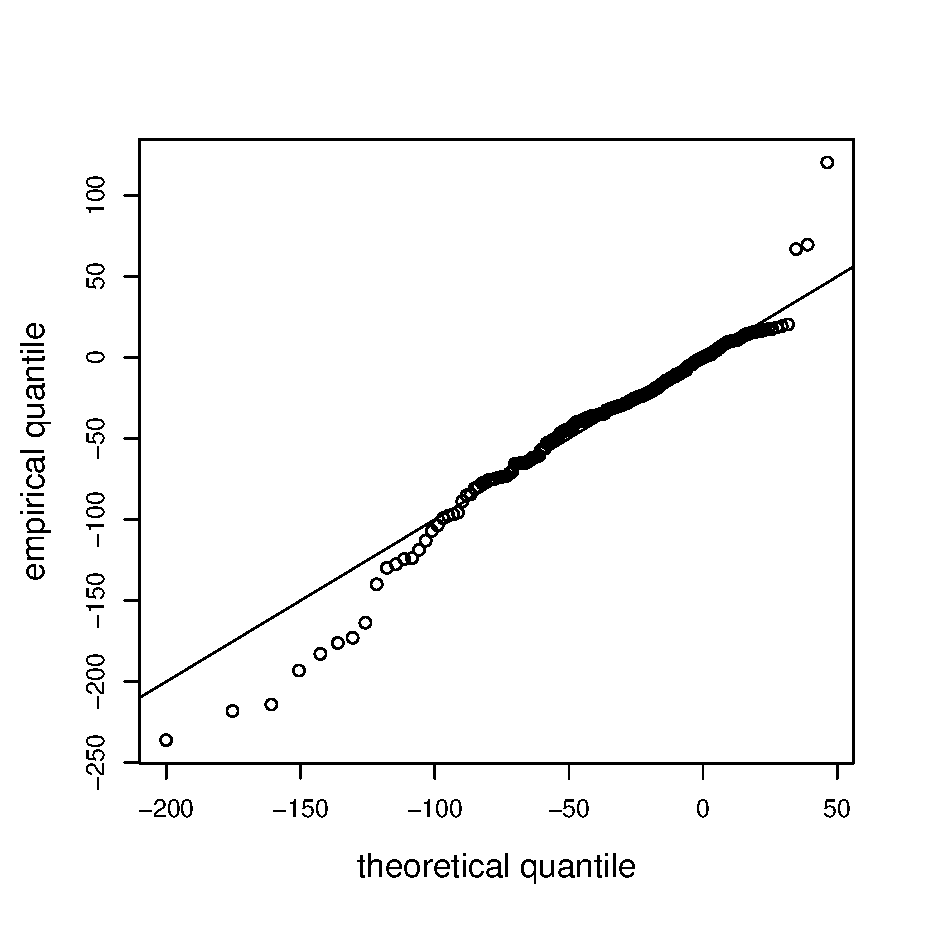
\includegraphics[width=0.45\textwidth]{Chapter17FatTail/F17GB2QQPlot.eps}
    \caption{\label{F17:GB2ResidAnalysis} Residual Analysis of the GB2 Model.
  The left-hand panel is a plot of residuals versus fitted values. The right-hand panel is a $qq$ plot of residuals.}
    \end{center}
\end{figure}\index{diagnostic checking!residual analysis}

\newpage

\section{Quantile Regression}\label{S17:QuantileReg}\index{regression model!quantile regression}

Quantile regression is an extension of median regression, so it is
helpful to introduce this concept first.

In median regression, one finds the set of regression coefficients
$\boldsymbol \beta$ that minimizes

\begin{equation*}
\sum_{i=1}^n | y_i - \mathbf{x}_i^{\prime} \boldsymbol \beta |.
\end{equation*}
That is, we simply replace the usual squared loss function with an
absolute value function. Although we will not go into the details
here, finding these optimal coefficients is a simple optimization
problem in nonlinear programming that can be readily implemented in
modern statistical software.

\index{least squares!least absolute deviations}

Because this procedure uses the absolute value as the loss function,
median regression is also known as \emph{LAD} for \emph{least
absolution deviations} as compared to \emph{OLS} (for ordinary least
squares). The adjective ``median'' comes from the special case where
there are no regressors so that $\mathbf{x}$ is a scalar 1. In this
case the minimization problem reduces to finding an intercept
$\beta_0$  that minimizes

\begin{equation*}
\sum_{i=1}^n | y_i - \beta_0 |.
\end{equation*}
The solution to this problem is the \emph{median} of $\{y_1, \ldots,
y_n\}$.

Suppose that you would also like to find the $25^{th}$, $75^{th}$,
or some other percentile of $\{y_1, \ldots, y_n\}$. One can also use
this optimization procedure to find any percentile, or
\emph{quantile}. Let $\tau$ be a fraction between 0 and 1. Then, the
$\tau$th sample quantile of $\{y_1, \ldots, y_n\}$ is the value of
$\beta_0$  that minimizes
\begin{equation*}
\sum_{i=1}^n \rho_{\tau}( y_i - \beta_0).
\end{equation*}
Here, $\rho_{\tau}(u)=u(\tau-{\rm I}(u\leq0))$ is called a
\emph{check function} and ${\rm I}(\cdot)$ is the indicator
function.

Extending this procedure, in quantile regression one finds the set
of regression coefficients $\boldsymbol \beta$ that minimizes
\begin{equation*}
\sum_{i=1}^n \rho_{\tau}( y_i - \mathbf{x}_i^{\prime} \boldsymbol
\beta ).
\end{equation*}
The estimated regression coefficients depend on the fraction $\tau$,
so we use the notation $\widehat{\boldsymbol \beta}(\tau)$ to
emphasize this dependence. The quantity
$\mathbf{x}_i^{\prime}\widehat{\boldsymbol \beta}(\tau)$ represents
the $\tau^{\rm th}$ quantile of the distribution of $y_i$ for the
explanatory vector $\mathbf{x}_i$. To illustrate, for $\tau = 0.5$,
$\mathbf{x}_i^{\prime}\widehat{\boldsymbol \beta}(0.5)$ represents
the estimated \emph{median} of the distribution of $y_i$. In
contrast, the $OLS$ fitted value $\mathbf{x}_i^{\prime}\mathbf{b}$
represents the estimated \emph{mean} of the distribution of $y_i$.

\linejed\index{datasets!nursing home utilization}

\textbf{Example: Wisconsin Nursing Homes - Continued.} To illustrate
quantile regression techniques, we fit a regression of square
footage (SqrFoot) on total person years (TPY). Figure
\ref{F17:QuanReg} shows the relationship between these two
variables, with mean (OLS) and median (LAD) fitted lines
superimposed. Unlike the original TPY distribution that is skewed,
for each value of SqrFoot we can see little difference between the
mean and median values. This suggests that the conditional
distribution of TPY given SqrFoot is not skewed.


Figure \ref{F17:QuanReg} also shows the fitted lines that result
from fitting quantile regressions at four additional values of $\tau
=0.05,0.25, 0.75$ and 0.95. These fits are indicated by the grey
lines. At each value of SqrFoot, we can visually get a sense of the
$5^{th}$, $25^{th}$, $50^{th}$, $75^{th}$, and $95^{th}$ percentiles
of the distribution of TPY. Although classic ordinary least squares
also provides this, the classic recipes generally assume
homoscedasticity. From \ref{F17:QuanReg}, we see that the
distribution of $y$ seems to widen as SqrFoot increases, suggesting
a heteroscedastic relationship.



\begin{figure}[htp]
  \centering
    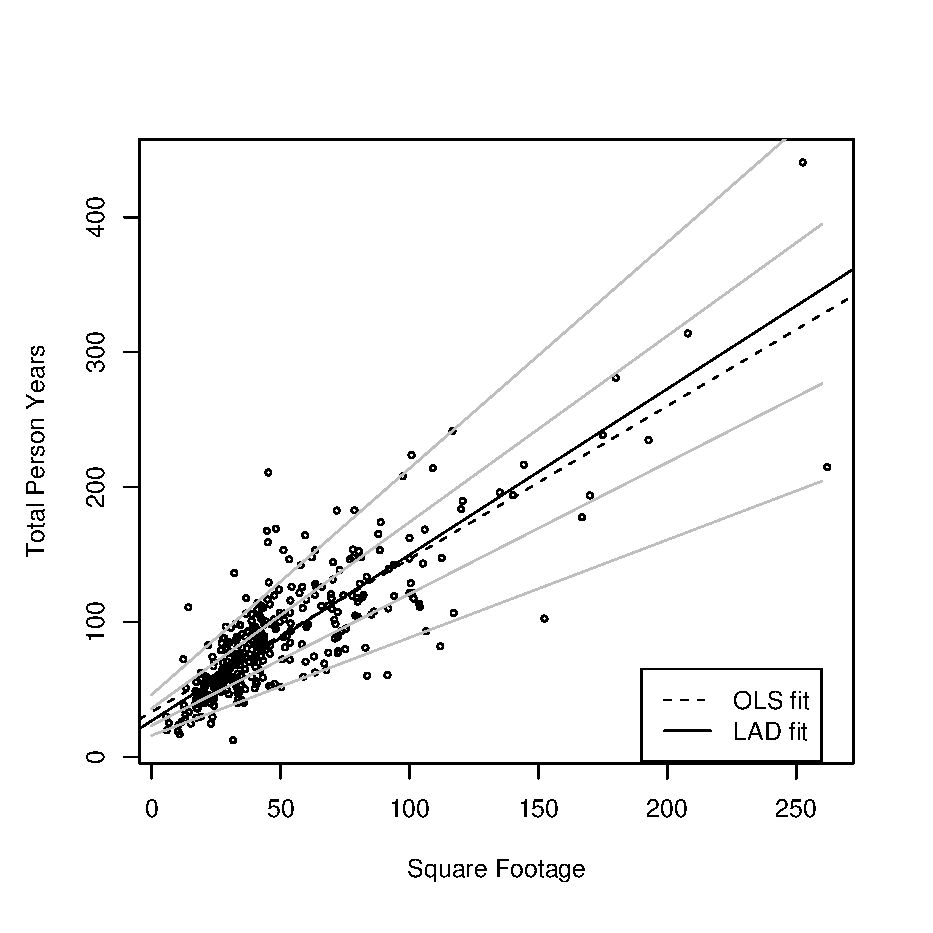
\includegraphics[width=.6\textwidth]
        {Chapter17FatTail/F17QuanReg.eps}
\caption{\label{F17:QuanReg} \small Quantile Regression Fits of
Square Footage on Total Person Years. Superimposed are fits from
mean (OLS) and median (LAD) regressions, indicated in the legend.
Also superimposed with grey lines are quantile regression fits --
from bottom to top, the fits correspond to $\tau =0.05,0.25, 0.75$
and 0.95.}
\end{figure}

\linejed

Quantile regressions perform well in situations when ordinary least
squares requires careful attention to be used with confidence. As
demonstrated in the Wisconsin Nursing Home example, quantile
regression handles skewed distributions and heteroscedasticity
readily. Just as ordinary quantiles are relatively robust to unusual
observations, quantile regression estimates are much less sensitive
to outlying observations than the usual regression routines.


\section{Extreme Value Models}\label{S17:ExtremeValueSection}

Extreme value models focus on the extremes, the ``tip of the
iceberg,'' such as the highest temperature over a month, the fastest
time to run a kilometer or the lowest return from the stock market.
Some extreme value models are motivated by maximal statistics.
Suppose that we consider annual chief executive officer (CEO)
compensation in a country, $y_1, y_2, \ldots$. Then, $M = \max(y_1,
\ldots, y_n)$ represents the compensation of the most highly paid
CEO during the year. If values $y$ were observed, then we could use
some mild additional assumptions (such as independence) to make
inference about the the distribution of $M$. However, in many cases,
only $M$ is directly observed, forcing us to base inference
procedures on ``extreme'' observations $M$. As a variation, we might
have observations for the top 20 CEO's -- not the entire population.
This variation uses inference based on the ``20'' largest order
statistics, see for example Coles (2003, Section 3.5.2).

\index{distributions!generalized extreme value, $GEV$}

Modeling $M$ is often based on the \textit{generalized extreme
value}, or $GEV$, distribution, defined by the distribution function
\begin{equation}\label{E17:GEV}
\Pr(M \leq x) = \exp \left[-(1+ \gamma z )^{-1/\gamma} \right],
\end{equation}
where $z=(x-\mu)/ \sigma$. This is a location-scale model, with
location and scale parameters $\mu$ and $\sigma$, respectively. In
the standard case where $\mu=0$ and $\sigma=1$, allowing $\gamma
\rightarrow \infty $ means that $\Pr(M \leq x) \rightarrow  \exp
\left[- e^{-x} \right],$ the classical extreme value distribution.
Thus, the parameter $\gamma$ provides the generalization of this
classical distribution.

Beirlant, Goegebeur, Segers and Teugels (2004) discuss ways in which
one could introduce regression covariates into the $GEV$
distribution, essentially by allowing each parameter to depend on
covariates. Estimation is done via maximum likelihood. In their
inference procedures, the focus is on the behavior of the extreme
quantiles (conditional on the covariates).

Another approach to modeling extreme values is to focus on data that
must be large to be included in the sample.

\linejed\index{examples!large medical claims}\index{truncated}


\textbf{Example: Large Medical Claims.} Cebri\'{a}n, Denuit and
Lambert (2003) analyzed 75,789 large group medical insurance claims
from 1991. To be included in this database, claims must exceed
\$25,000. Thus, these data are left-truncated at \$25,000. The
interest in their study was to interpret the long-tailed
distribution in terms of covariates age and sex.

\linejed

The \emph{peaks over threshold} approach to modeling extremes values
is motivated by left-truncated data where the truncation point, or
``threshold,'' is large. To be included in the data set, the
observations must exceed a large threshold that we refer to as a
``peak.'' Following our Section 14.2 discussion on truncation, if
$C_L$ is the left truncation point, then the distribution function
of $y-C_L$ given that $y>C_L$ is $1 - \Pr(y-C_L > x |y>C_L) = 1 -
(1-F_y(C_L+x))/(1-F_y(C_L))$. Instead of modeling the distribution
of $y$, $F_y$, directly as in prior sections, one assumes that it
can be directly approximated by a \emph{generalized Pareto
distribution}. That is, we assume
\begin{equation}\label{E17:GPD}
\Pr(y-C_L \leq x |y>C_L) \approx 1 - (1+ \frac{z}{\theta}
)^{-\theta} ,
\end{equation}
where $z=x / \sigma$, $\sigma$ is a scale parameter, $x \geq 0$ if
$\theta \geq 0$ and $ 0 \leq x \leq - \theta$ if $\theta < 0$. Here,
the right-hand side of equation (\ref{E17:GPD}) is the generalized
Pareto distribution. The usual Pareto distribution restricts
$\theta$ to be positive; this specification allows for negative
values of $\theta$. Allowing $\theta \rightarrow 0 $ means that $1 -
(1+ z/\theta )^{-\theta} \rightarrow 1 - e^{-x/\sigma},$ the
exponential distribution.

\index{distributions!Pareto}\index{distributions!generalized Pareto
distribution}


\linejed


\textbf{Example: Large Medical Claims - Continued.} To incorporate
age and sex covariates, Cebri\'{a}n et al. (2003) categorized the
variables, allowed parameters to vary by category and estimated each
category in isolation of the others. Alternative, more efficient,
approaches are described in Chapter 7 of Beirlant et al. (2004).

\linejed


\bigskip


\section{Further Reading and References}

The literature on long-tailed claims modeling is actively
developing. A standard reference is Klugman et al (2008). Kleiber
and Kotz (2003) provide an excellent survey of the univariate
literature, with many historical references. Carroll and Ruppert
(1988) provide extensive discussions of transformations in
regression modeling.

This chapter has emphasized the GB2 distribution with its many
special cases. Venter (2007) discusses extensions of the generalized
linear model, focusing on loss reserving applications. Balasooriya
and Low (2008) provide a recent applications to insurance claims
modeling, although without any regression covariates. Another
approach is to use a skewed elliptical (such as a normal or $t$-)
distribution. Bali and Theodossiou (2008) provide a recent
application, showing how to use such distributions in time series
modeling of stock returns.

Koenker (2005) is an excellent book-long introduction to quantile
regression. Yu, Lu and Stander (2003) provide an accessible shorter
introduction.

Coles (2003) and Beirlant et al. (2004) are two excellent book-long
introductions to extreme value statistics.



\bigskip

\textbf{References}


\scalefont{0.9}

\begin{multicols}{2}

Balasooriya, Uditha and Chan-Kee Low (2008). Modeling insurance
claims with extreme observations: Transformed kernel density and
generalized lambda distribution. \emph{North American Actuarial
Journal} 11(2) 129-142.

Bali, Turan G. and Panayiotis Theodossiou (2008). Risk measurement
of alternative distribution functions. \emph{Journal of Risk and
Insurance} 75(2), 411-437.

Beirlant, Jan, Yuir Goegebeur, Robert Verlaak and Petra Vynckier
(1998). Burr regression and portfolio segmentation.
\textit{Insurance: Mathematics and Economics} 23, 231-250.

Beirlant, Jan, Yuir Goegebeur, Johan Segers and Jozef Teugels
(2004). \emph{Statistics of Extremes}. Wiley, New York.

Burbidge, J.B. and Magee, L. and Robb, A.L. (1988). Alternative
transformations to handle extreme values of the dependent variable.
\textit{Journal of the American Statistical Association} 83,
123-127.

Carroll, Raymond and David Ruppert (1988). \textit{Transformation
and Weighting in Regression}. Chapman-Hall.

Cebri\'{a}n, Ana C., Michel Denuit and Philippe Lambert (2003).
Generalized Pareto fit to the Society of Actuaries' large claims
database. \emph{North American Actuarial Journal} 7 (3), 18-36.

Coles, Stuart (2003). \emph{An Introduction to Statistical Modeling
of Extreme Values}. Springer, New York.

Cummins, J. David, Georges Dionne, James B. McDonald and B. Michael
Pritchett (1990). Applications of the GB2 family of distributions in
modeling insurance loss processes. \textit{Insurance: Mathematics
and Economics} 9, 257-272.

John, J. A. and Norman R. Draper (1980). An alternative family of
transformations. \textit{Applied Statistics} 29 (2), 190-197.

Kleiber, Christian  and Samuel Kotz (2003). \textit{Statistical Size
Distributions in Economics and Actuarial Sciences}. John Wiley and
Sons, New York.

Klugman, Stuart A, Harry H. Panjer and Gordon E. Willmot (2008).
\emph{Loss Models: From Data to Decisions}. John Wiley \& Sons,
Hoboken, New Jersey.

Koenker, Roger (2005). \textit{Quantile Regression}. Cambridge
University Press, New York.

Manning, William G (1998). The logged dependent variable,
heteroscedasticity, and the retransformation problem.
\textit{Journal of Health Economics} 17, 283-295.

Manning, William G, Anirban Basu and John Mullahy (2005).
Generalized modeling approaches to risk adjustment of skewed
outcomes data. \emph{Journal of Health Economics} 24, 465�488.

McDonald, James B. and Richard J. Butler (1990). Regression models
for positive random variables. \textit{Journal of Econometrics} 43,
227-251.

Rachev, Svetiozar, T., Christian Menn and Frank Fabozzi (2005).
\textit{Fat-Tailed and Skewed Asset Return Distributions:
Implications for Risk Management, Portfolio Selection, and Option
Pricing}. Wiley, New York.

Rosenberg, Marjorie A., Edward W. Frees, Jiafeng Sun, Paul Johnson
and James M. Robinson (2007). Predictive modeling with longitudinal
data: A case study of Wisconsin nursing homes. \emph{North American
Actuarial Journal} 11(3), 54-69.

Sun, Jiafeng, Edward W. Frees and Marjorie A. Rosenberg (2008).
Heavy-tailed longitudinal data modeling using copulas.
\textit{Insurance: Mathematics and Economics} 42(2), 817-830.

Venter, Gary (2007). Generalized linear models beyond the
exponential family with loss reserve applications. \textit{Astin
Bulletin: Journal of the International Actuarial Association} 37
(2), 345-364.

Yeo, In-Kwon and Richard A. Johnson (2000). A new family of power
transformations to improve normality or symmetry.
\textit{Biometrika} 87, 954-959.

Yu, Keming, Zudi Lu and Julian Stander (2003). Quantile regression:
applications and current research areas. \textit{Journal of the
Royal Statistical Society Series D (The Statistician)}  52 (3),
331-350.


\end{multicols}


\scalefont{1.1111}


\section{Exercises}

\begin{exercises}

\scalefont{0.90}

\item Quantiles and Simulation. Use equation (\ref{E17:GenDistEq}) to establish the
following distributional relationships that are helpful for
calculating quantiles.

a. Assume that $y_0 = \alpha_1 F/\alpha_2$ where $F$ has an
$F$-distribution with numerator and denominator degrees of freedom
$df_1 = 2 \alpha_1$ and $df_2 = 2 \alpha_2$. Show that $y$ has a GB2
distribution.

b. Assume that $y_0 = B/(1-B),$ where $B$ has a beta distribution
with parameters $\alpha_1$ and $\alpha_2$. Show that $y$ has a GB2
distribution.

c. Describe how to use parts (a) and (b) for calculating quantiles.

d. Describe how to use parts (a) and (b) for simulation.


\item Consider a GB2 probability density function given in equation
(\ref{E17:GB2}).

a. Reparameterize the distribution by defining the new parameter
$\theta =e^{\mu }.$ Show that the density can be expressed as:
\begin{equation*}
\mathrm{f}_{GB2}(y;\theta, \sigma ,\alpha _1,\alpha _2)=\frac{\Gamma
\left( \alpha _1+\alpha _2\right) }{\Gamma \left( \alpha _1\right)
\Gamma \left( \alpha _2\right) }\frac{\left( y/\theta \right)
^{\alpha _2/\sigma }}{\sigma y\left[ 1+\left( y/\theta \right)
^{1/\sigma }\right] ^{\alpha _1+\alpha _2}},
\end{equation*}

b. Using part (a), show that
\begin{equation*}
\lim_{\alpha _2\rightarrow \infty }\mathrm{f}_{GB2}(y; \theta \alpha
_2^{\sigma },\sigma ,\alpha _1,\alpha _2)=\frac{1}{\sigma y\Gamma
\left( \alpha _1\right) }\left( y/\theta \right) ^{\alpha _1/\sigma
}\exp \left( -\left( y/\theta \right) ^{1/\sigma }\right)
=\mathrm{f}_{GG}(y;\theta, \sigma, \alpha _1),
\end{equation*}
a generalized gamma density.

c. Using part (a), show that
\begin{equation*}
\mathrm{f}_{GB2}(y;\theta, \sigma, 1, \alpha_2)=\frac{\alpha
_2\left( y/\theta \right) ^{\alpha _2/\sigma }}{\sigma y\left[
1+\left( y/\theta \right) ^{1/\sigma }\right] ^{1+\alpha
_2}}=\mathrm{f}_{Burr}(y;\theta, \sigma, \alpha _2),
\end{equation*}
a Burr Type 12 density.


\item Recall that the density of a gamma distribution with shape
parameter $\alpha $\ and scale parameter $\theta $ has a density
given by $\mathrm{f}(y)=\left[ \theta ^{\alpha }\Gamma \left( \alpha
\right) \right] ^{-1}y^{\alpha -1}\exp
\left( -y/\theta \right) $\ and k$^{th}$ moment given by $\mathrm{E}%
(y^{k})=\theta ^{k}\Gamma \left( \alpha +k\right) /\Gamma \left(
\alpha \right) $, for $k>-\alpha .$


a. For the GB2 distribution, show that
\begin{equation*}
\mathrm{E}(y)=e^{\mu }\frac{\Gamma \left( \alpha _1+\sigma \right)
\Gamma \left( \alpha _2-\sigma \right) }{\Gamma \left( \alpha
_1\right) \Gamma \left( \alpha _2\right) }.
\end{equation*}

b. For the generalized gamma distribution, show that
\begin{equation*}
\mathrm{E}(y)=e^{\mu }\Gamma \left( \alpha_1 +\sigma \right) /\Gamma
\left( \alpha_1 \right) .
\end{equation*}

c. Calculate the moments of a Burr Type 12 density.



\scalefont{1.1111}

\end{exercises}
